\documentclass[ignoreonframetext,unicode]{beamer}

\usepackage[utf8]{inputenc}
\usepackage[T1]{fontenc}
\usepackage[english,russian]{babel}
\usepackage{amsmath}
\usepackage{amsfonts}
\usepackage{amssymb}
\usepackage{graphicx,pgf}
\usepackage{multimedia}

\usetheme{Warsaw}

\useinnertheme{circles}   %внутренняя тема
%\useoutertheme{smoothbars}   %внешняя тема
\usecolortheme{seahorse}     %цветовая схема
%\usefonttheme{serif}    %шрифты
%\defbeamertemplate*{footline}{shadow theme}
%\setbeameroption{hide notes}

%номера слайдов
\newcommand*\oldmacro{}%
\let\oldmacro\insertshorttitle%
\renewcommand*\insertshorttitle{%
	\oldmacro\hfill%
	\insertframenumber\,/\,\inserttotalframenumber}
\RequirePackage{caption}
\DeclareCaptionLabelSeparator{defffis}{ }
\captionsetup{justification=centering,labelsep=defffis}

%\title{Курсовая работа}
%\subtitle{Численные схемы для аппроксимации неограниченных решений при моделировании обтекания профиля крыла в вихревых методах}
\title[Уравнение изгиба балки]{Нахождения уравнения изгиба балки}
\author[Пиневич В.\,Г.]{Докладчик: Пиневич В.\,Г.\and\\[0.5mm] Научный руководитель: Чередниченко А.\,В.}

\institute[каф. Прикладная математика ФН-2]{группа ФН2-41Б}
\date{\today}
\titlegraphic{
\includegraphics[width=2cm]{logo.png}}
%\renewcommand{\vec}[1]{\text{\mathversion{bold}${#1}$}}


\begin{document}
	
	\begin{frame}[plain]
		\maketitle
		%\insertshortinstitute{Группа ФН2-41Б}
	\end{frame}

	\begin{frame}{Условия равновесия}
		\begin{columns}
			\column{\textwidth}\vspace*{-2.0mm}
			\begin{block}{Состояния равновесия}\vspace*{-3.5mm}
			 \[
			 	\begin{cases}
			 	\sum\limits {{F_z = 0}} \\
			 	\sum\limits {{M_z = 0}}
			 \end{cases}
			 \Leftrightarrow
			 \begin{cases}
			 	Q + q dz - Q - Q dz = 0 \\
			 	M + Q dz + q dz \frac {dz}{z} - M -dM = 0
			 \end{cases}
			 \]
			\end{block}
			
			\begin{block}{Получаем итоговые условия равновесия}	
			\[
			\begin{cases}
				\frac {dQ}{dz} = q \\
				\frac {dM}{dz} = Q
			\end{cases}
			\]
			\end{block}

		
		Равно распределенная нагрузка
		\begin{columns}
			\column{0.5\textwidth}
			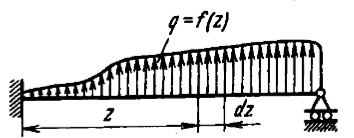
\includegraphics[width=\textwidth]{pic.1.1}
			\column{0.5\textwidth}
			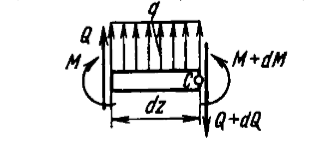
\includegraphics[width=\textwidth]{pic.1.2}
		\end{columns}

		\end{columns}
		
	\end{frame}

		\begin{frame}{Чистый изгиб}
				\begin{block}{Условия чистого изгиба}	
				\[
				\mbox{Только изгибающие моменты, }
				Q = 0, M = const
				\]
			\end{block}
			
		Сечение балки
		\begin{columns}
			\column{0.5\textwidth}
			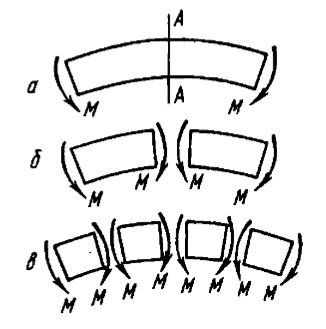
\includegraphics[width=\textwidth]{pic.2}
		\end{columns}
		\end{frame}

	\begin{frame}{Деформация сечения}
		Рассмотрим деформацию как поворот плоских поперечных сечений относительно друг друга. Слой который не изменится при изгибе --- нейтральный.
		\begin{columns}
			\column{0.45\textwidth}
			\begin{block}{Кривизна нейтрального слоя}	
				\[
				\frac {1}{\rho} = \frac {d\theta}{dz}
				\]
			\end{block}
			\column{0.55\textwidth}
			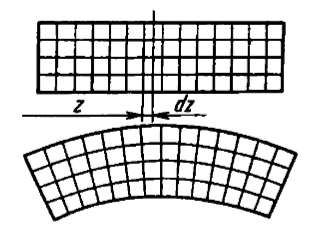
\includegraphics[width=\textwidth]{pic.3}
		\end{columns}
	\end{frame}

	\begin{frame}{Относительное удлинение и напряженность}
		
	\begin{columns}	
		\column{0.55\textwidth}
	Случайный отрезок $AB = dz$ получит приращение $A'B' - AB$. \\
	С учетом того, что сечение остается плоским,\\ $A'B' - AB = (\rho + y)d\theta - \rho d\theta = yd\theta$, где $y$ --- расстояние от $AB$ до $CD$. 
	\column{0.55\textwidth}
	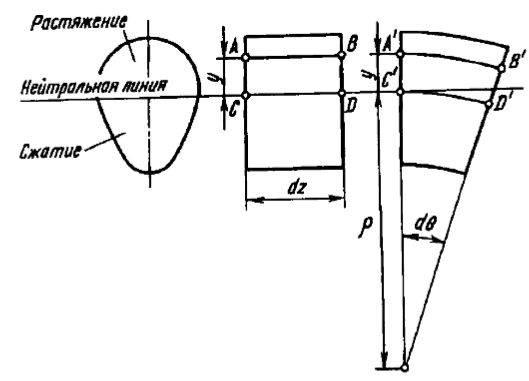
\includegraphics[width=\textwidth]{pic.4}
	\end{columns}
	\begin{columns}
		\column{0.5\textwidth}
		\begin{block}{Относительное удлинение $AB$}	
			\[
			\varepsilon = \frac {y d\theta}{dz} = \frac{y}{\rho}
			\]
		\end{block}
		\column{0.5\textwidth}
		\begin{block}{Напряженность}	
			\[
			\sigma = E \varepsilon = E \frac{y}{\rho}
			\]
		\end{block}
	\end{columns}
	\end{frame}

	\begin{frame}{Изгибающий момент}
	Изгибающий момент в поперечном сечении стержня может быть выражен через напряжения $\sigma$. \\ Момент сил $\sigma d F$ относительно оси $y$ равен нулю, а относительно $x$ -- полному изгибающему моменту $M$.
	\begin{columns}
		\column{0.5\textwidth}
		\begin{block}{Изгибающий момент $M_y$}	
			\[
			M_y = \int_{F} \sigma x d F = \frac{E}{\rho} \int_{F} y x d F = 0
			\]
		\end{block}
		\column{0.55\textwidth}
		\begin{block}{Изгибающий момент $M_x$}	
			\[
			M_x = \int_{F} \sigma y d F = \frac{E}{\rho} \int_{F} \sigma y^2 d F = M
			\]
		\end{block}
	\end{columns}
	
		\begin{block}{Зависимость кривизны стержня от изгибающего момента}	
		\[
		\frac{1}{\rho} = \frac{M}{E J_{x}}
		\]
		\end{block}
	\end{frame}

		\begin{frame}{Дифференциальное уравнение равновесия стержня}
		\begin{columns}
			\column{0.45\textwidth}
			\begin{block}{Форма изогнутого стержня}	
				\[
				\frac{1}{\rho} = \frac{y''}{(1 + y'^2)^{\frac{3}{2}}} \approx y''
				\]
			\end{block}
			\column{0.6\textwidth}
			\begin{block}{Дифференциальное уравнение балки}	
				\[
				y'' = \frac{M}{E J_{x}}
				\]
			\end{block}
		\end{columns}
	
		\begin{columns}
			\column{0.25\textwidth}
		\begin{block}{Угол поворота}
			\[
			\theta = y'
			\]
		\end{block}
			\column{0.25\textwidth}
		\begin{block}{Момент}
			\[
			M = E J_{x} y''
			\]
		\end{block}

			\column{0.25\textwidth}
		\begin{block}{Точечная сила}
			\[
			Q = E J_{x} y'''
			\]
		\end{block}
		\column{0.25\textwidth}
		\begin{block}{Распр. нагрузка}
			\[
			q_{y} = E J_{x} y^{IV}
			\]
		\end{block}
	
		\end{columns}
	
	\end{frame}

\section{Теоретическая часть}

	\begin{frame}{Метод начальных коэффициентов}
		Представим полученные выражения в виде системы. Учитывая граничные условия, решаем ее, получаем уравнение прогиба стержня $y(z)$.
	
	\begin{block}{}	
		\[
		\begin{cases}
			\frac{d Q}{d z} - q_{y}(z) = 0\\
			\frac {d M}{d z} - Q = 0\\
			\frac{d \theta}{d z} - \frac{M}{E J_{x}(z)} = 0\\
			\frac{d y}{d z} - \theta = 0 
		\end{cases}
		\]
	\end{block}
	\end{frame}


	\begin{frame}{Метод обобщенных коэффициентов}
		\begin{block}{Функция Дирака}	
			\[
			\int_{-\infty}^z \delta (z - a) \varphi (z) dz = 
			\begin{cases}
				\infty, z = a \\
				0, z \neq a	
			\end{cases}
			\]
		\end{block}
		
		\begin{columns}
			\column{0.4\textwidth}
			Возможное представление функции Дирака
			\column{0.6\textwidth}
			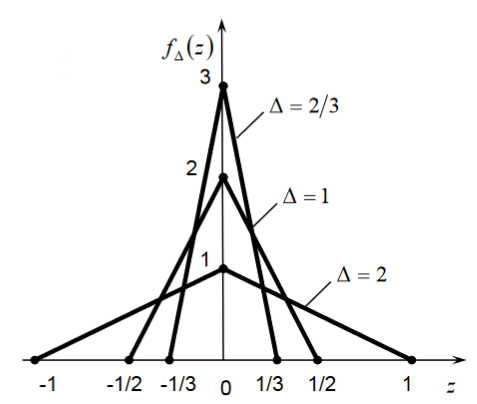
\includegraphics[width=\textwidth]{dirac}
		\end{columns}
		
		
	\end{frame}

	\begin{frame}{Метод обобщенных коэффициентов}
		\begin{block}{Функция Хевисайда}	
			\[
			H(z - a) = 
			\begin{cases}
				0, z < a \\
				1, z \geqslant a	
			\end{cases}
			\]
		\end{block}
	Единичная функция Хевисайда

	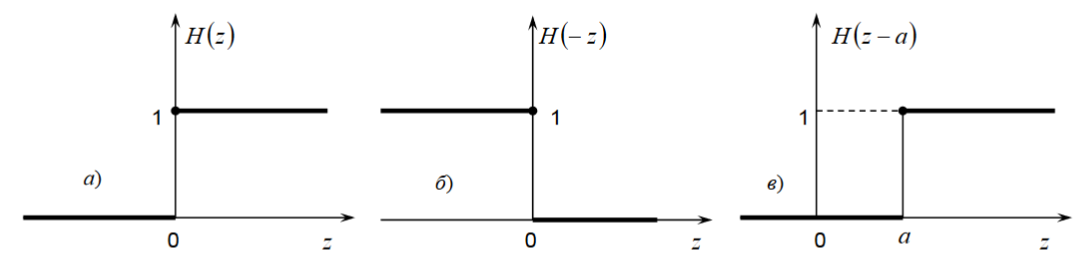
\includegraphics[width=1\textwidth]{heavi}
		
	\end{frame}


\begin{frame}{Метод обобщенных коэффициентов}
	
	\begin{block}{Связь функций Дирака и Хевисайда}	
		\[
		\int_{-\infty}^z \delta (z - a) dz = 
		H(z)
		\]
	\end{block}

	\begin{block}{Интегрирование функции Дирака}	
	\[
	\int_0^z f(z) \delta(z - a) d z = f(a)H(z - a)
	\]
	\end{block}

	\begin{block}{Интегрирование функции Хевисайда}	
	\[
	\int_0^z f(z) H(z - a) d z = H(z - a)\int_a^z f(z) d z
	\]
	\end{block}

\end{frame}

	\begin{frame}{Интегрирование функции Хевисайда}
		
		\begin{columns}
			\column{0.4\textwidth}
			Интеграл функции Хевисайда
			\column{0.55\textwidth}
			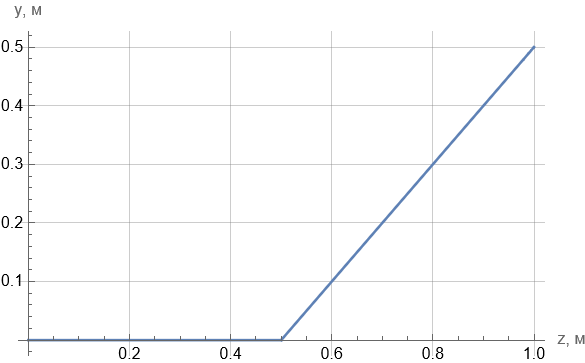
\includegraphics[width=\textwidth]{intHeav}
		\end{columns}
		
		\begin{columns}
			\column{0.4\textwidth}
			Повторный интеграл функции Хевисайда
			\column{0.55\textwidth}
			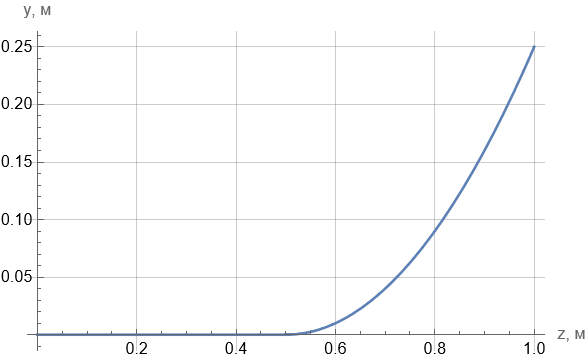
\includegraphics[width=\textwidth]{int2Heav}
		\end{columns}

	\end{frame}

\section{Решение задач}

	\begin{frame}{Балка в заделке}
	\textbf{Задача.} Составить уравнение упругой линии в заделке, нагруженной на конце сосредоточенной силой $P = 1$ Н. 
	$E_{Al} = 70$~ГПа, $ J_{x} = \frac{l h^3}{12}$~$\mbox{кг} \cdot \mbox{м}^2$, $h = 0.01$~м, $l = 1$~м.
	
	\begin{center}
		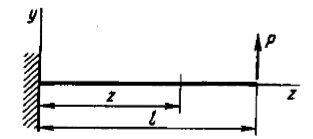
\includegraphics[width=0.6\textwidth]{pic.7}
	\end{center}
	
	\end{frame}

	\begin{frame}{Решение методом начальных коэффициентов}

		\begin{block}{Граничное условие}
		\[
		y = 0;\mbox{ } \theta = 0\mbox{, при } z = 0
		\]		
		\end{block}

	\begin{enumerate}
	\item Найдем момент $M = \int\limits_z^l P d z = P(l - z)$
	
	\item Далее ищем угол наклона сечения $\theta$:
	\begin{gather*}
	\theta = \frac{P}{E J_{x}} \int\limits_z^l (l - z)d z = \frac{P}{E J_{x}} (\frac{z^2}{2} - l z + c_1)
	\end{gather*}

		\item Получаем уравнение изгиба балки:
	\begin{gather*}
		y = \frac{P}{E J_{x}} \int\limits_z^l (\frac{z^2}{2} - l z + c_1) d z = \frac{P}{E J_{x}} (\frac{z^3}{6} - \frac{z^2 l}{2} + c_1 z + c_2)
	\end{gather*}

	\end{enumerate}
\end{frame}

	\begin{frame}{Решение методом начальных коэффициентов}
Найдем $c_1$ и $c_2$. Из граничных условий следует, что $c_1 = 0$, поскольку $y(0) = 0$, а $c_2 = 0$, так как $\theta(0) = 0$.
\begin{columns}
	\column{0.35\textwidth}  
\begin{block}{Итоговое уравнение}	
	\[
	y = \frac{P}{E J_{x}} (\frac{z^3}{6} - \frac{z^2 l}{2})
	\]
\end{block}
\column{0.65\textwidth}  
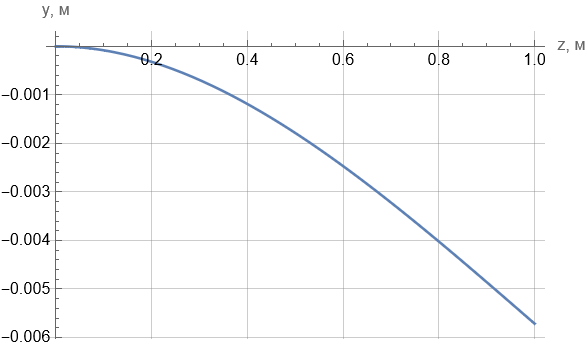
\includegraphics[width=\textwidth]{g.1}
\end{columns}
\end{frame}

	\begin{frame}{Решение методом обобщенных коэффициентов}
	
	\begin{block}{Граничное условие}
		\[
		y = 0;\mbox{ } \theta = 0\mbox{, при } z = 0
		\]		
	\end{block}
	
	\begin{enumerate}
		\item С помощью ф-ии Дирака запишем: $E J_{x} y^{IV} = P \delta (z)$
		
		\item Интегрируем:
		$
			E J_{x} y''' = P H (z)
		$
		
		\item Еще раз интегрируем:
		$
			P \int_l^z  H (z) dz = P H (z) (z - l)
		$
		
		\item Найдем угол поворота балки:
		\begin{gather*}
			E J_{x} y' = P \int_l^z P H (z) (z - l) dz = P H(z)(\frac{z^2}{2} - l z) + c_1
		\end{gather*}
	
	\item Получаем уравнение гибкого изгиба балки:
	\begin{gather*}
		y = \frac{P}{E J_{x}} (\frac{z^3}{6} - \frac{z^2 l}{2}) H(z) + c_1 z + c_2
	\end{gather*}
		
	\end{enumerate}
\end{frame}

\begin{frame}{Решение методом обобщенных коэффициентов}
	Из граничных условий получаем: $c_1 = 0, c_2 = 0.$ Учитывая, что $H(z) = 1 \mbox{, при } z \leqslant l$, получаем ответ.
	\begin{columns}
		\column{0.35\textwidth}  
		\begin{block}{Итоговое уравнение}	
			\[
		y = \frac{P}{E J_{x}} (\frac{z^3}{6} - \frac{z^2  l}{2})
			\]
		\end{block}
		\column{0.65\textwidth}  
		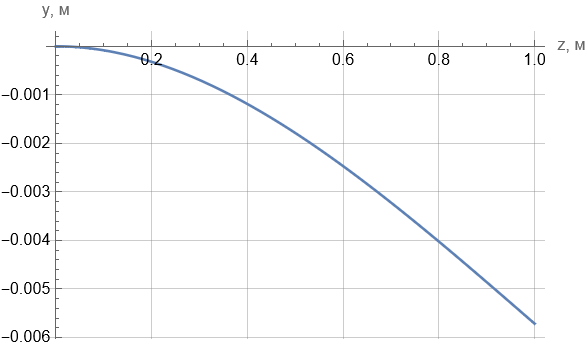
\includegraphics[width=\textwidth]{g.1}
	\end{columns}

\begin{center}
	{Таким образом, графики двух методов совпали.}
\end{center}
\end{frame}

	\begin{frame}{Двух опорная балка}
	\textbf{Задача.} Двух опорный стержень длинной $l$ нагружен силой $P = 1$ Н, расположен на расстоянии a от левой опоры~(рис. \ref{pic8}). Составить уравнение упругой линии. 
	\newline 
	$E_{Al} = 70$~ГПа, $J_{x} = \frac{l h^3}{12}$~$\mbox{кг} \cdot \mbox{м}^2$, $h = 0.01$~м, $l = 1$~м.
	
	\begin{center}
		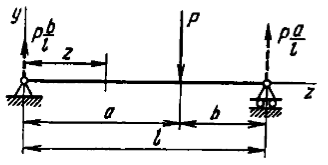
\includegraphics[width=0.6\textwidth]{pic.8}
	\end{center}
	
\end{frame}

	\begin{frame}{Решение методом начальных коэффициентов}
	
	\begin{block}{Граничное условие}
		\[
		\begin{cases}
			y_1 = 0 \mbox{, при } z = 0\\
			y_2 = 0 \mbox{, при } z = l\\
			y_1 = y_2 \mbox{, при } z = a
		\end{cases}
		\]		
	\end{block}
	Разобьем стержень на 2 части: до точки приложения $P$ и после.
	\begin{enumerate}
		\item  Сила $Q_1 = \frac{P b}{l} $.
		
		\item Найдем момент $M_1 = \frac{b}{l} \int\limits_0^z P d z = P z + c_0^1$. Параметр $c_0^1 = 0$, так как момент равен нулю
		
		\item Найдем угол поворота $\theta_1$:
		\begin{gather*}
				\theta_1 = \frac{b}{l} \frac{P}{E J_{x}} \int\limits_0^z P z d z = \frac{b}{l} \frac{P}{E J_{x}} (\frac{b}{l} \frac{z^2}{2} + c_1^1)
		\end{gather*}		
	\end{enumerate}
\end{frame}

\begin{frame}
	Получаем первое уравнение изгиба балки $y_1$:
	\begin{gather*}
		y_1 = \frac{b}{l} \frac{P}{E J_{x}} \int\limits_0^z (\frac{z^2}{2} + \theta_1) dz =  \frac{b}{l} \frac{P}{E J_{x}} (\frac{z^3}{6} + c_1^1 z + c_2^1)
	\end{gather*}
Параметр $c_2^1 = 0$, так как концах стержень неподвижен по оси $y$. 
\end{frame}

\begin{frame}
	Рассмотрим вторую часть стержня. 
	\begin{enumerate}
		\item Сила $Q_2 = \frac{P a}{l}$.
		
		\item Найдем момент $M_2 = \frac{a}{l} \int\limits_l^z P d z = -P(z + l)$
		
		\item Найдем угол поворота $\theta_2$:
		\begin{gather*}
			\theta_2 = - \frac{a}{l} \frac{P}{E J_{x}} \int\limits_l^z P(z + l) d z = - \frac{a}{l} \frac{P}{E J_{x}} (\frac{z^2}{2} + z l - c_1^2)
		\end{gather*}
		
		\item Получаем второе уравнение изгиба балки $y_2$: 
		\begin{gather*}
			y_2 =  - \frac{a}{l} \frac{P}{E J_{x}} \int\limits_l^z (\frac{z^2}{2} + z l - c_1^2) dz = - \frac{a}{l}  \frac{P}{E J_{x}} (\frac{z^3}{6} + \frac{z^2 l}{2} - c_1^2 z + c_2^2)
		\end{gather*}
	\end{enumerate}
\end{frame}

\begin{frame}
	Из граничных условий получаем:
		\begin{columns}
		\column{0.5\textwidth}  
		\begin{block}{}	
			\[
			\begin{cases}
				c_2^1 = 0\\
				c_2^2 = a^3 \frac{1}{6}
			\end{cases}
			\]
		\end{block}
		\column{0.5\textwidth}  
				\begin{block}{}	
			\[
			\begin{cases}
				y_1 = y_2\\
				y_1' = y_2'
			\end{cases}
			\]
		\end{block}
	\end{columns}
\vspace*{2mm}
Решаем систему, подставляем параметры в уравнение $y_1$ и $y_2$.
\begin{block}{Итоговые уравнения}
	\[
		y(z) = 
	\begin{cases}
		y_1 = \frac{P}{6 E J_{x}} \frac{b}{l} (z^3 - \frac{2}{3} z l(2 l - \frac{2}{3}l))\mbox{, при } 0 \leqslant z \leqslant a\\
		y_2 = \frac{P}{6 E J_{x}} \frac{a}{l} (-z^3 + 3 z^2 l - z(2 l^2 + \frac{4}{9} l^2) + \frac{4}{9}l^4)\mbox{, иначе }
	\end{cases}
\]
\end{block}

\end{frame}

\begin{frame}{Решение методом начальных коэффициентов}
	\begin{columns}
		\column{0.35\textwidth}  
		Пусть $a = \frac{2 l}{3}, b = \frac{l}{3}$, тогда уравнение изгиба балки будет иметь следующий график
		\column{0.65\textwidth}  
		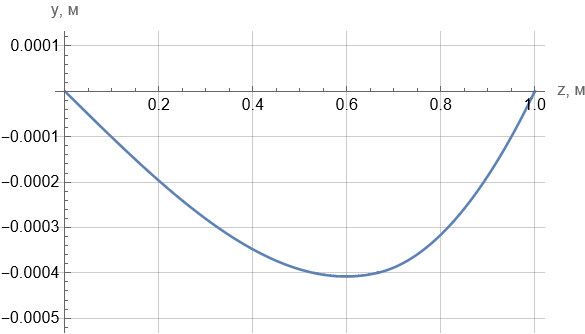
\includegraphics[width=\textwidth]{g.2}
	\end{columns}
\end{frame}

\begin{frame}{Решение методом обобщенных коэффициентов}
	
	\begin{block}{Граничное условие}
		\[
		\begin{cases}
			y = 0, M = 0 \mbox{, при } z = 0\\
			y = 0, M = 0 \mbox{, при } z = l.
		\end{cases}
		\]		
	\end{block}
	
	\begin{enumerate}
		\item С помощью ф-ии Дирака запишем: $E J_{x} y^{IV} = P \delta (z)$
		
		\item Интегрируем:
		$
		E J_{x} y''' = P H (z)
		$
		
		\item Еще раз интегрируем:
		$
		M = P \int_l^z  H (z) dz = P H (z) (z - l)
		$
		
		\item Найдем угол поворота балки:
		\begin{gather*}
			y = \frac{P}{E J_{x}} (\frac{z^3}{6} - \frac{z^2 l}{2}) H(z) + c_1 z + c_2
		\end{gather*}
		
		\item Получаем уравнение гибкого изгиба балки:
		\begin{gather*}
			y = \frac{P}{E J_{x}} (\frac{z^3}{6} - \frac{z^2 l}{2}) H(z) + c_1 z + c_2
		\end{gather*}
		
	\end{enumerate}
\end{frame}

\begin{frame}{Решение методом обобщенных коэффициентов}
	Из граничных условий
	\begin{gather*}
		c_2 = 0, c_1 = \frac{P l(3 a^2 z^2 - 3 a l z + l^2)}{6 a^3 E J_{x}}.
	\end{gather*}
	Кроме того, $H(z) = 1 \mbox{, при } z \leqslant l$. 
	
		\begin{block}{Итоговое уравнение}	
			\[
			y = \frac{P}{E J_{x}} (-\frac{z^3}{6} \frac{1}{a} + \frac{(z - \frac{l}{a})^3}{6} H(z - \frac{l}{a}) + \frac{l(3 a^2 z^2 - 3 a l z + l^2)}{6 a^3})
			\]
		\end{block}
\end{frame}

\begin{frame}{Решение методом обобщенных коэффициентов}
	\begin{columns}
		\column{0.35\textwidth}  
		Пусть $a = \frac{2 l}{3}, b = \frac{l}{3}$, тогда уравнение изгиба балки будет иметь следующий график
		\column{0.65\textwidth}  
		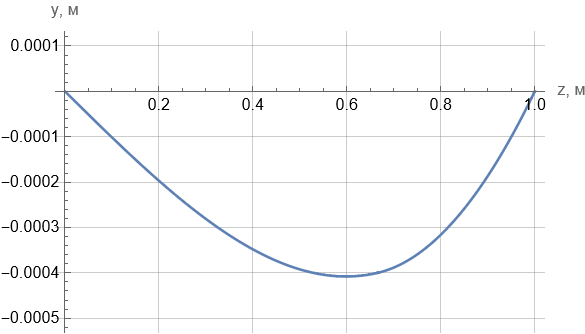
\includegraphics[width=\textwidth]{g.4}
	\end{columns}
\begin{center}
{Таким образом, графики двух методов совпали.}
\end{center}
\end{frame}

\begin{frame}{Результаты}
	В ходе работы получены следующие результаты
	\begin{block}{}
	\begin{enumerate}
		\item Изучены методы начальных коэффициентов и обобщенных функций нахождения уравнения упругого изгиба стержня.	
		\item Решены 2 типа задач с помощью этих методов, их результат оказался идентичны.
		\item Метод начальных коэффициентов является более трудоемким и менее удобным по сравнению с методом обобщенных функций, поскольку требует учета большего количества граничных условий, больший объем вычислений.
	\end{enumerate}
	\end{block}	
\end{frame}	
\end{document} 